\documentclass[tombow,dvipdfmx]{corona-a5-1.1}
% dvipdfmxを追加(川口)

% Springer document settings
\usepackage[bottom]{footmisc}% places footnotes at page bottom

\usepackage{newtxtext}       % 
\usepackage[varvw]{newtxmath}       % selects Times Roman as basic font
%%%%%%%%%%%%%%%%%%%%%%%%%%%%%%%

% \usepackage{amssymb}
\usepackage{ntheorem}
\usepackage{amsmath}
\usepackage{enumitem}


\usepackage{graphicx}
\usepackage{color}
\usepackage{cite}
\usepackage{makeidx}


\usepackage{ascmac}
\usepackage{eclbkbox}
\usepackage{dsfont}

\usepackage{longtable}

\usepackage{url}

\usepackage{hyperref}

\usepackage{multicol}

%% --川口追加--
\makeatletter
\let\MYcaption\@makecaption
\makeatother
\usepackage{subcaption}
\captionsetup{compatibility=false}      % 必要に応じて

\makeatletter
\let\@makecaption\MYcaption
\makeatother
% ----

%%
\theoremstyle{plain}
\theoremheaderfont{\bfseries}
\theorembodyfont{\rmfamily}
\theoremseparator{\hspace{1ex}}
\theoremindent0cm
\theoremnumbering{arabic}
\theoremprework{\vspace{1ex}\begin{shadebox}\vspace{1ex}}
\theorempostwork{\vspace{-1ex}\end{shadebox}\vspace{1ex}}

%%
\theoremclass{theorem}

%%
\theoremclass{theorem}

%%
\theoremclass{theorem}


%%
\theoremstyle{break}
\theoremheaderfont{\bfseries}
\theorembodyfont{\rmfamily}
\theoremseparator{}
\theoremindent0cm
\theoremnumbering{arabic}
\theoremprework{\vspace{1.5ex}\begin{breakbox}\vspace{-0.5ex}}
\theorempostwork{\vspace{-0.5ex}\end{breakbox}\vspace{1.5ex}}

%%
\theoremstyle{nonumberplain}
\theoremseparator{\hspace{1ex}}

%%
\newtheorem{assumption}{Assumption}[section]

%%
\renewcommand{\theproblem}{}

\renewcommand{\theremark}{}


\newcommand{\red}[1]{{\color{red}#1}}
\newcommand{\blue}[1]{{\color{blue}#1}}
\newcommand{\green}[1]{{\color{green}#1}}

\DeclareMathOperator*{\argmax}{arg\,max}

\newcommand{\bm}[1]{\boldsymbol{#1}}
\newcommand{\sfT}{\mathsf{T}}

\newcommand{\advanced}{$^{\ddag}$}

\DeclareMathOperator{\sfsin}{\mathsf{sin}}
\DeclareMathOperator{\sfcos}{\mathsf{cos}}
\DeclareMathOperator{\sftan}{\mathsf{tan}}
\DeclareMathOperator{\sfarctan}{\mathsf{arctan}}

\DeclareMathOperator{\sfdiag}{\mathsf{diag}}
\DeclareMathOperator{\sfcol}{\mathsf{col}}
\DeclareMathOperator{\sfdet}{\mathsf{det}}
\DeclareMathOperator{\sfadj}{\mathsf{adj}}
\DeclareMathOperator{\sftrace}{\mathsf{trace}}

\DeclareMathOperator{\real}{\mathsf{Re}}

\DeclareMathOperator{\sfker}{\mathsf{ker}}
\DeclareMathOperator{\sfim}{\mathsf{im}}

\DeclareMathOperator{\sfdim}{\mathsf{dim}}
\DeclareMathOperator{\sfspan}{\mathsf{span}}

\DeclareMathOperator{\sfint}{\mathsf{int}}

\DeclareMathOperator*{\sfmin}{\mathsf{min}}
\DeclareMathOperator*{\sfmax}{\mathsf{max}}
\DeclareMathOperator*{\sfsup}{\mathsf{sup}}

\DeclareMathOperator{\sfsat}{\mathsf{sat}}

\newcommand{\mat}[1]{\left[\: \begin{matrix} #1 \end{matrix} \:\right]}
\newcommand{\spliteq}[1]{\begin{split} #1 \end{split}}
\newcommand{\simode}[1]{\begin{cases}  \begin{split} #1 \end{split} \end{cases}}

\newcommand{\proofend}{\hfill \rule{2mm}{3mm}}

\newcommand{\Xti}{X_i'}
\newcommand{\Xsi}{X_i}

\newcommand{\Xtone}{X_1'}
\newcommand{\XtN}{X_N'}

\newcommand{\Xt}{X'}
\newcommand{\Xs}{X}

\newcommand{\taudi}{\tau_i}
\newcommand{\taud}{\tau}

\newcommand{\Cgi}{b_i}


\newcommand{\Ifd}{I_{\rm field} }

\newcommand{\matlab}{\textsc{Matlab} }





%% --川口追加--
\newcommand{\thshift}{\theta_{12}}
\newcommand{\thshiftb}{\theta_{32}}
\newcommand{\Ysa}{\bm y_{12}}
\newcommand{\bca}{c_{12}}
\newcommand{\Ysb}{\bm y_{32}}
\newcommand{\bcb}{c_{32}}
\newcommand{\bcij}{c_{ij}}
\newcommand{\Is}{{\bm I}_{12}' }
\newcommand{\im}{\bm j}
\newcommand{\tr}{{\sf T}}

%%%%%%%%%%%%%%%%%%%%%%%%% code lines %%%%%%%%%%%%%%%%%%%%%%%%%%%%%%%%%%%%%%%%%%
\usepackage{listings}
\usepackage{xcolor}
\renewcommand{\lstlistingname}{Program}% Listing -> Algorithm
\renewcommand{\lstlistlistingname}{List of \lstlistingname s}% List of Listings -> List of Algorithms

\definecolor{codegreen}{rgb}{0,0.6,0}
\definecolor{codegray}{rgb}{0.5,0.5,0.5}
\definecolor{codepurple}{rgb}{0.58,0,0.82}
\definecolor{backcolour}{rgb}{0.95,0.95,0.92}

\lstdefinestyle{mystyle}{
    backgroundcolor=\color{backcolour},   
    commentstyle=\color{codegreen},
    keywordstyle=\color{magenta},
    numberstyle=\tiny\color{codegray},
    stringstyle=\color{codepurple},
    basicstyle=\ttfamily\footnotesize,
    breakatwhitespace=false,         
    breaklines=true,                 
    captionpos=b,                    
    keepspaces=true,                 
    numbers=left,                    
    numbersep=5pt,                  
    showspaces=false,                
    showstringspaces=false,
    showtabs=false,                  
    tabsize=2
}

\lstset{style=mystyle}

\begin{document}

\chapter{Numerical simulation example of a large-scale model}\label{chap:largesim}
\red{Entire chapter translated with DeepL}

In this chapter, we apply the basic items explained so far to perform numerical simulation of a standard large-scale model called the IEEE68 bus system model.
The structure of this chapter is as follows.
First, in the \ref{sec: IEEE68} section, the numerical data of the transmission line, load, and generator of the IEEE68 bus system model are organized.
Next, in the \ref{sec: IEEE68AGC} section, the effect of automatic power generation control on load fluctuations is analyzed.
Specifically, we analyze changes in generator variables and bus variables when the impedance of the load changes slowly over several hours.
Finally, in the \ref{sec: IEEE68PSS} clause, the transient stability for the generatrix ground fault is analyzed.
In particular, based on the retrofit control theory, it is shown that the system stability is appropriately improved by incorporating an independently designed system stabilizer into each generator.


\section{Target power system model}\label{sec:IEEE68}

\begin{figure}[t]
\centering
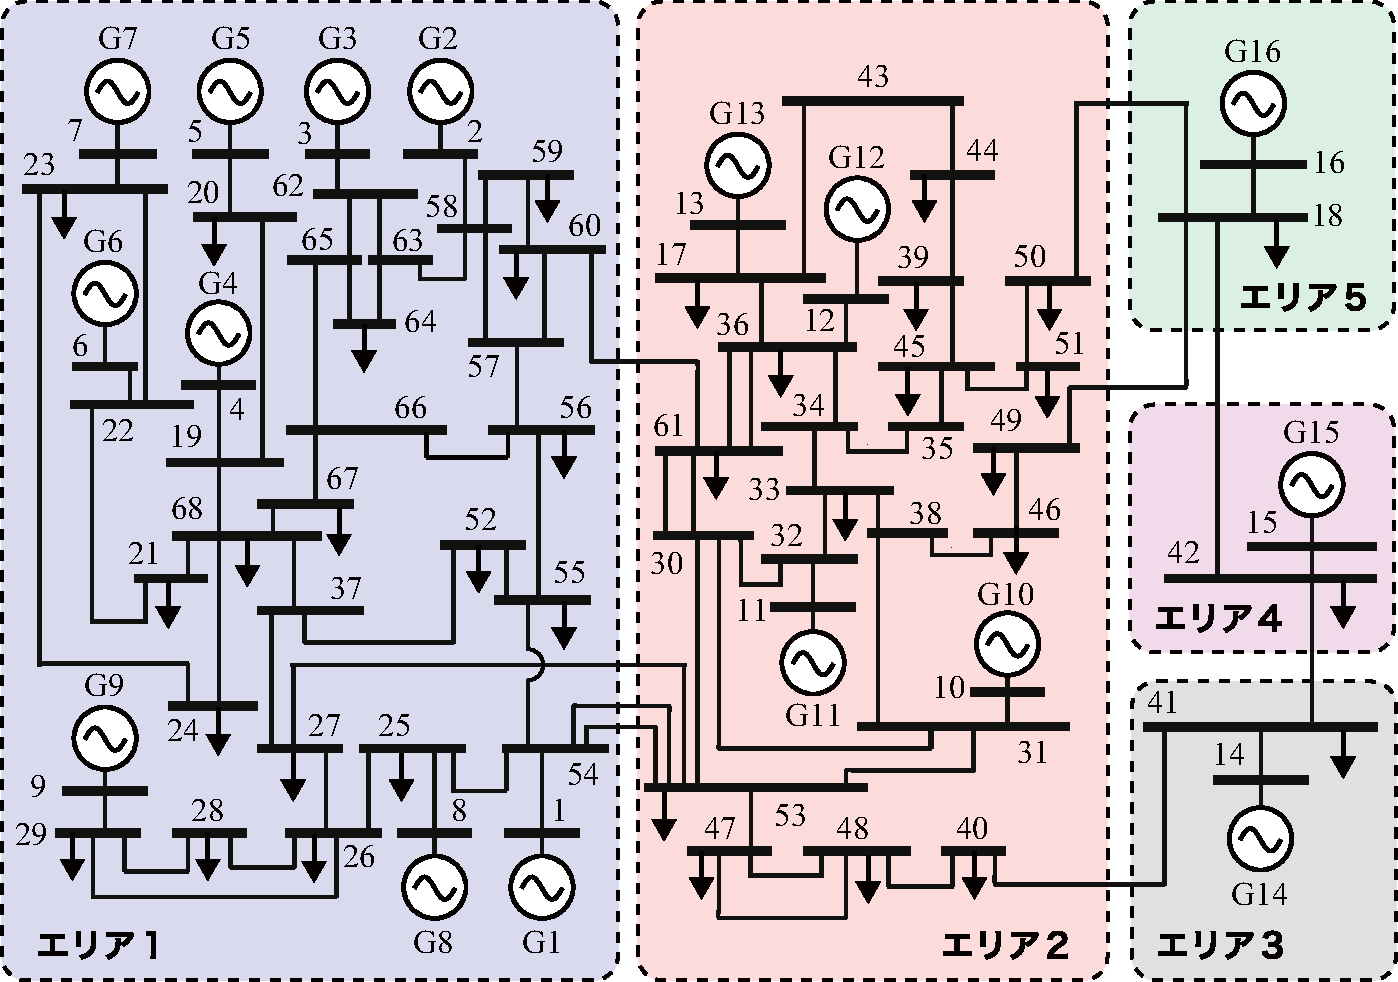
\includegraphics[width = .99\linewidth]{figs/IEEE68bus}
\medskip
\caption{\textbf{IEEE68 bus system model}}
\label{fig:IEEE68bus}
\medskip
\end{figure}

\subsection{IEEE68 bus system model}

This section exemplifies the numerical simulation results using the IEEE68 bus system model (\FIGref{fig: IEEE68bus}).
This model consists of 68 bus lines, of which 16 bus bars are connected to the generator and 35 bus bars are connected to the load.
In \FIGref{fig: IEEE68bus}, "Area 1" represents the power system in the New England region of the northeastern United States, and "Area 2" represents the power system in New York.
Areas 3 to 5 represent the power systems around New York State as a set of generators and loads, respectively.

The transmission line is set as a model considering the ground capacitance explained in the \ref{sec: transmodc} section.
Set the constant of each transmission line to the value of \TABref{table: ieee68lines}.
The first column shows the bus number at the end of the transmission line, and the second, third, and fourth columns show the resistance, reactance, and capacitance to ground of the transmission line, respectively.
These are the standard values shown in \cite[Appendix A]{pal2006robust}.
For the generator, the salient pole type generator model explained in the \ref{sec: genmodadv} section is adopted.
Set the constant of each generator to the value of \TABref{table: ieee68genpara}.
These are also the values shown in the above literature.

\subsection{Data sheet used for tidal current calculation}


The data sheet of the generator bus used for power flow calculation is shown in \TABref{table: ieee68datag}.
Similarly, the data sheet of the load bus is shown in \TABref{table: ieee68datal}.
These also quote the values shown in \cite[Appendix A]{pal2006robust}.


\subsection{Load model}

The constant impedance model explained in the \ref{sec: loadpr} section is adopted as the load model.
For the data sheets of \TABref{table: ieee68datag} and \TABref{table: ieee68datal}, the impedance value of the load determined from the result of the power flow calculation is \TABref{table: ieee68loads}.
Note that the bus 16 is set as the slack bus, and the value of $ P_ {16} ^ {\ star} $ is calculated to be 33.68.

\section{Frequency stability analysis for load fluctuations}\label{sec:IEEE68AGC}

\subsection{Load fluctuation settings}

In this section, we observe the time response of the angular frequency deviation when the impedance value of the load is changed.
The load impedance is linearly increased by 10 \% per hour based on the value of \TABref{table: ieee68loads}.
That is, the impedance of each load is
\begin{align}\label{eq:loadvary68}
z_{{\rm load}i}(t) = \left(1+\tfrac{1}{36000}t \right) \left( r_{{\rm load}i} + \bm{j} x_{{\rm load}i} \right)
\end{align}
The unit of time $ t $ is [s].

\subsection{When the machine input and field input of the generator are constant}\label{sec:constPV}

Consider the case where the machine input and the field input, which are the external inputs of the generator, are all constants.
Angular frequencies for all generators when the load impedance changes according to the equation \ref{eq: loadvary68} from the steady-state to the datasheets of \TABref{table: ieee68datag} and \TABref{table: ieee68datal}. The time response of the deviation is shown in \FIGref{fig: omegasAGC}(a).
In this case, it can be seen that the angular frequency deviation does not become 0 because the supply-demand balance is not satisfied when the load fluctuates.
In addition, the angular frequency deviation increases in the negative direction for the first 7 seconds due to the increase in power consumption due to the increase in the impedance value of the load, and then the power system model becomes unstable and diverges in the positive direction. is doing.

\begin{figure}[t]
  \centering
  {
  \begin{minipage}{0.49\linewidth}
    \centering
    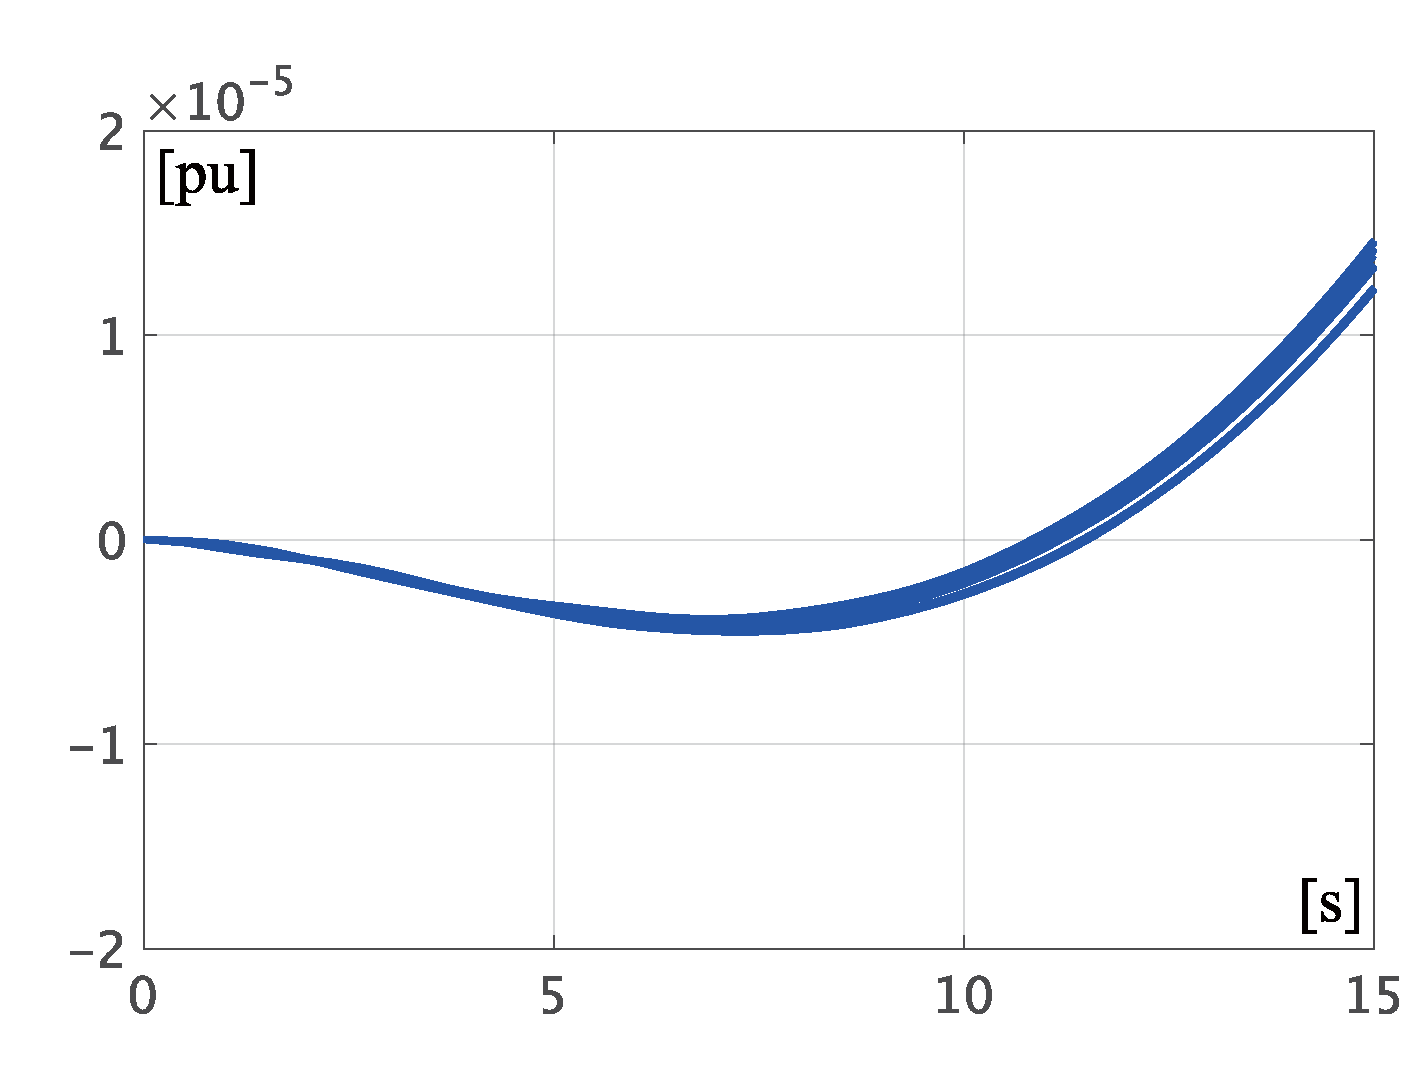
\includegraphics[width = 1.0\linewidth]{figs/WOavrWOagc}
    \subcaption{When machine input and field input are constants}
    \medskip
  \end{minipage}
  \begin{minipage}{0.49\linewidth}
    \centering
    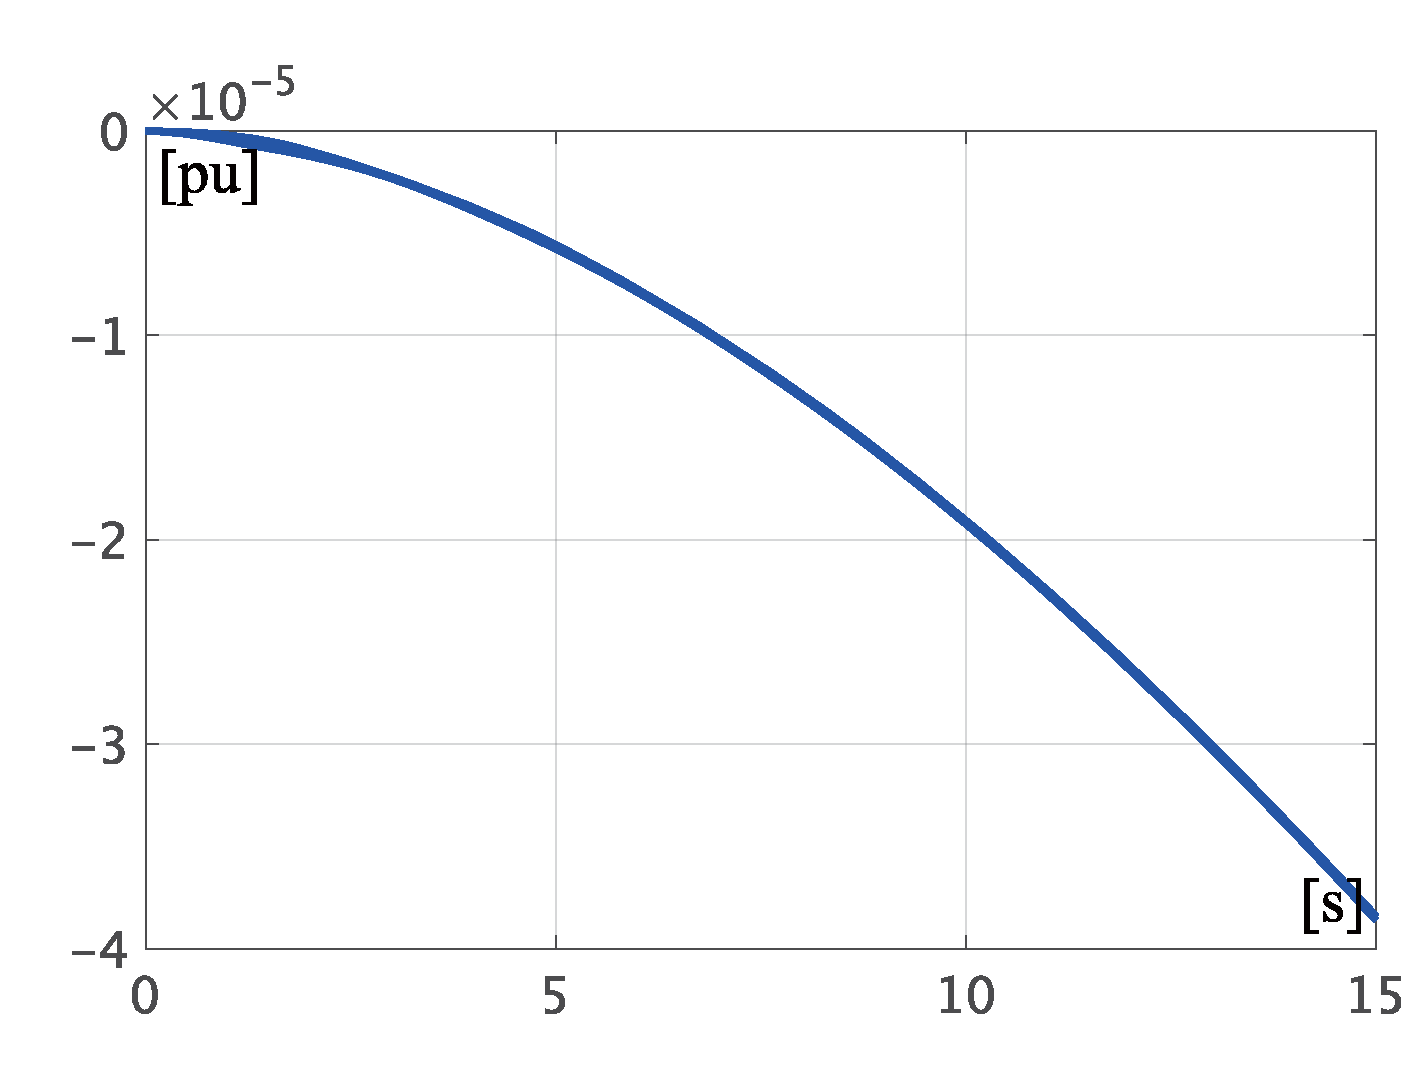
\includegraphics[width = 1.0\linewidth]{figs/WavrWOagc}
    \subcaption{If the machine input is a constant}
    \medskip
  \end{minipage}
 \begin{minipage}{0.49\linewidth}
    \centering
    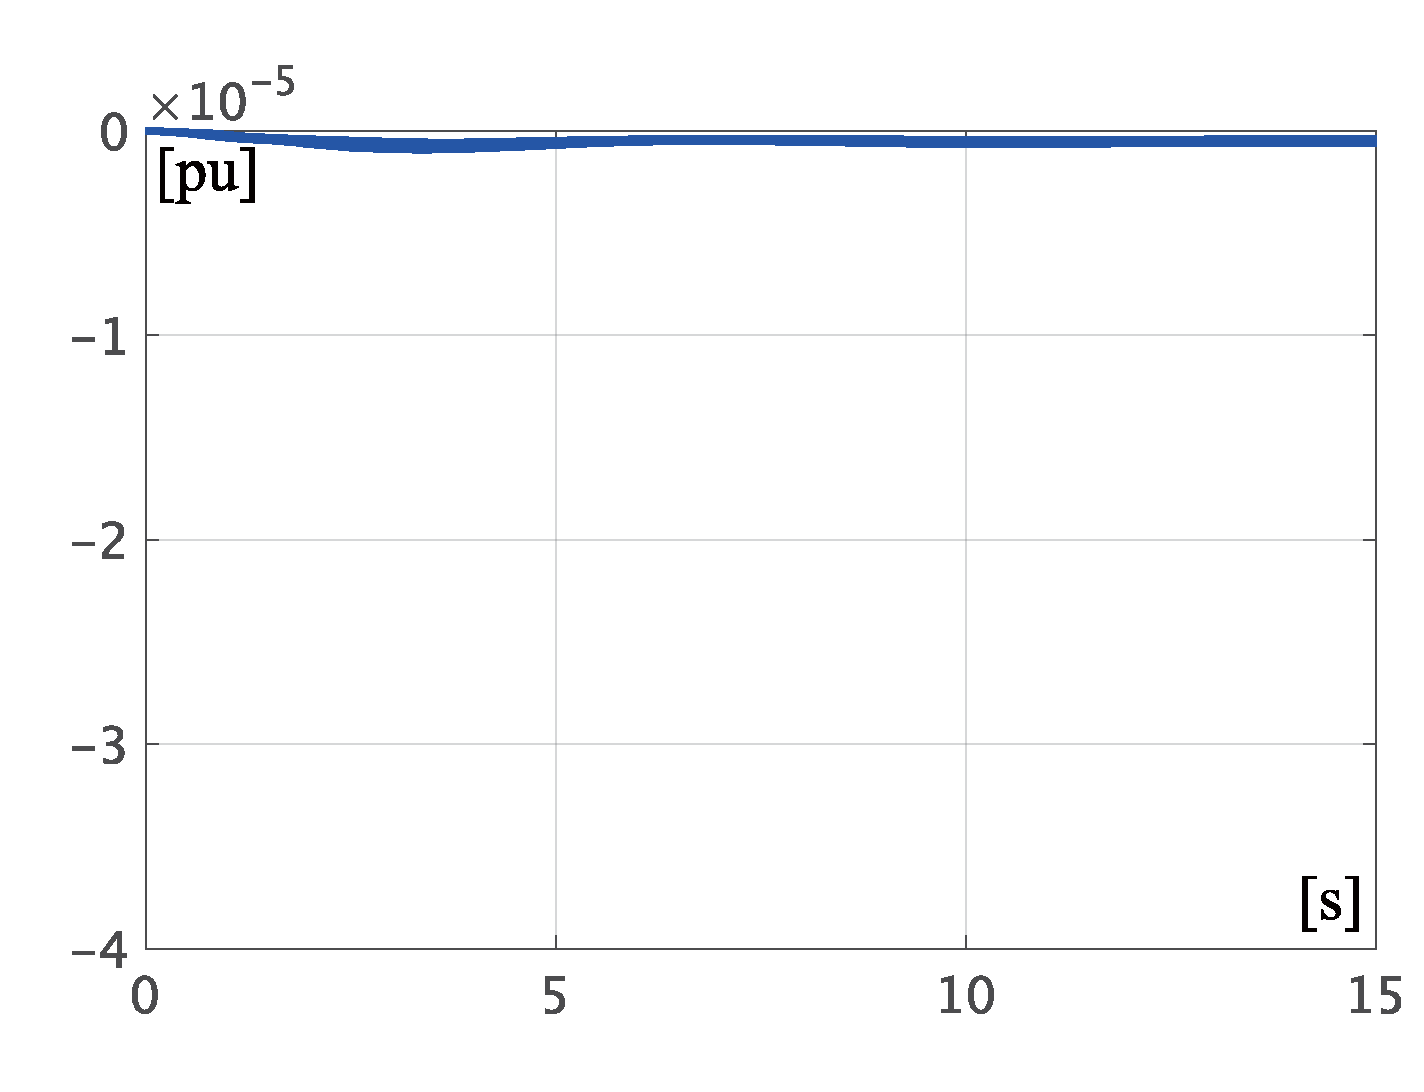
\includegraphics[width = 1.0\linewidth]{figs/WavrWagc}
    \subcaption{To control machine inputs}
    \medskip
  \end{minipage}
  \begin{minipage}{0.49\linewidth}
    \centering
    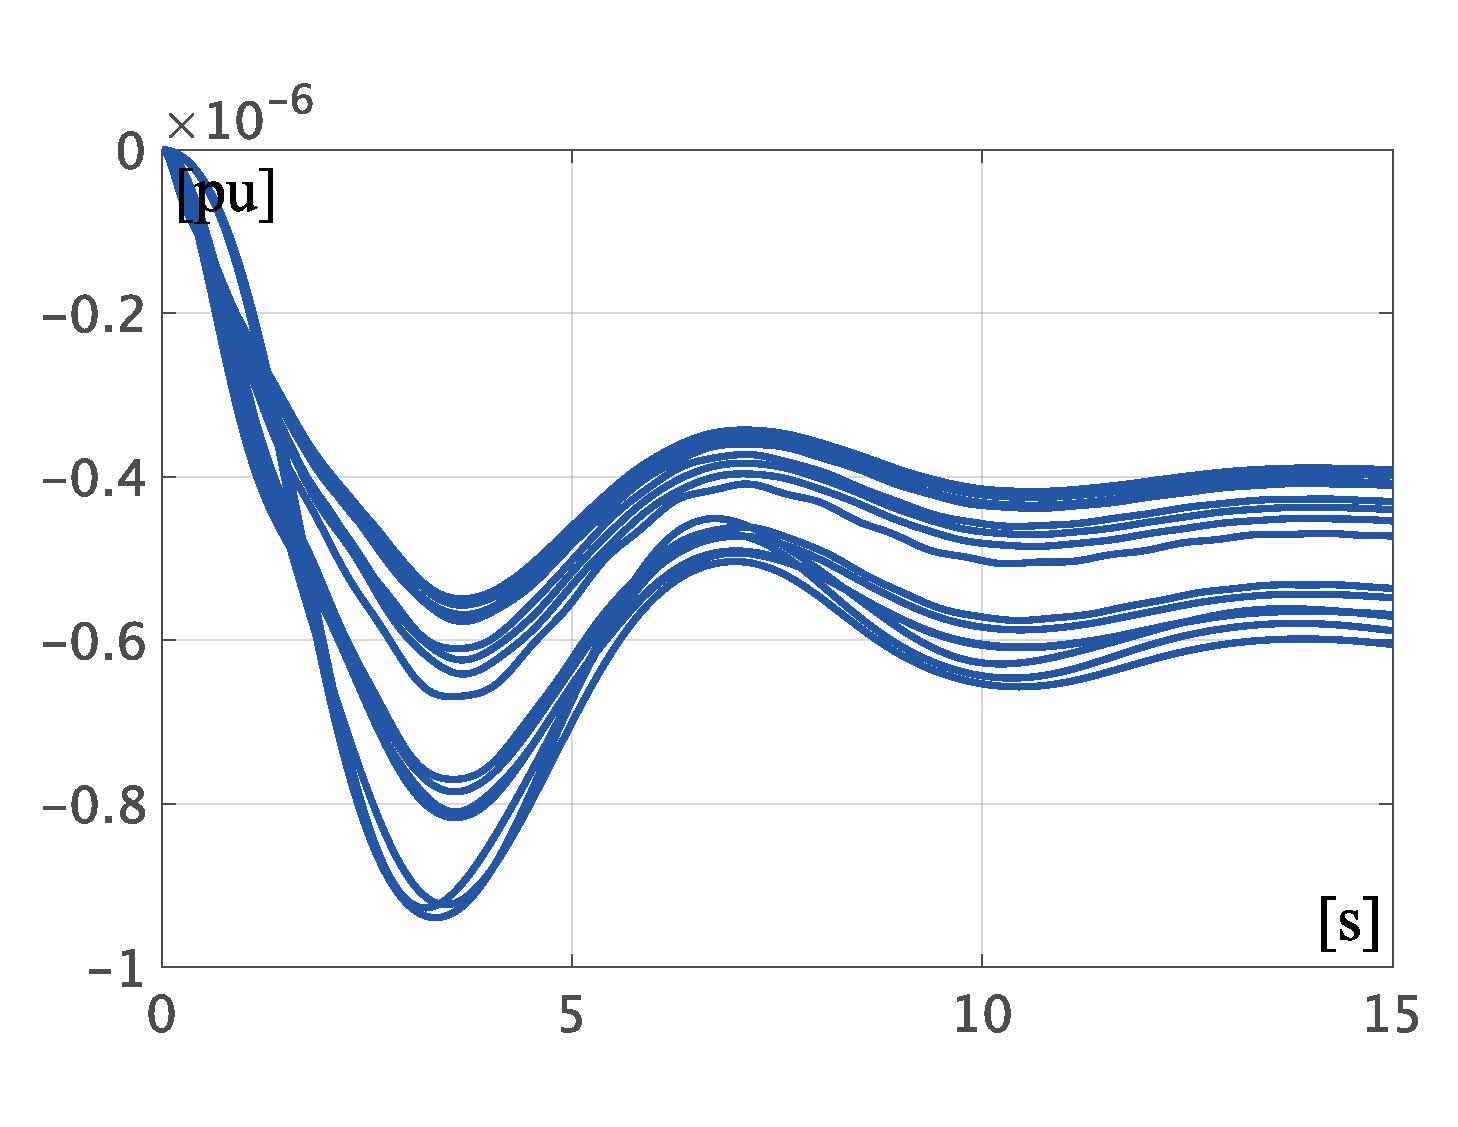
\includegraphics[width = 1.0\linewidth]{figs/WavrWagcL}
    \subcaption{When controlling machine inputs (zoom in)}
    \medskip
  \end{minipage}
  }
  \medskip
  \caption{\textbf{Time response of angular frequency deviation to load variations}}
  \label{fig:omegasAGC}
\medskip
\end{figure}


%\begin{table}[h]
%\medskip
%%\caption{\textbf{潮流計算に用いるデータシート(発電機母線)}} \label{table:xxx}
% \centering
%  {
%  \begin{minipage}{0.64\linewidth}
% \caption{\textbf{IEEE ST1型モデルのパラメータ}}
% \label{table:AVRparaset}
% \centering
%  \begin{tabular}{ccccccccc}
%   \hline
%$\tau_{\rm tr}$ & $\tau_{\rm ap}$ & $k_{\rm ap}$ & $\gamma_{+}$ & $\gamma_{-}$ & $k_{0}$ & $\tau_{\rm st}$ & $k_{\rm st}$\\
%   \hline \hline
% 0.015 & 0 & 20 & $\infty$ & $-\infty$ & 0 & 0 & 0 \\
%   \hline
%  \end{tabular}
%  \end{minipage}
%  \begin{minipage}{0.35\linewidth}
% \caption{\textbf{自動発電制御のパラメータ}}
% \label{table:agcparaset}
% \centering
%  \begin{tabular}{ccccccccc}
%   \hline
%  $k_{\rm P}$ & $k_{\rm I}$ & $\alpha_i$  \\
%   \hline \hline
%100 & 500 & 1  \\
%   \hline
%  \end{tabular}
%  \end{minipage}
%  }
%\end{table}



%\begin{table}[h]
%\medskip
% \caption{\textbf{自動発電制御のパラメータ設定}}
% \label{table:agcparaset}
% \centering
%  \begin{tabular}{ccccccccc}
%   \hline
%  $k_{\rm P}$ & $k_{\rm I}$ & $\alpha_i$  \\
%   \hline \hline
%100 & 500 & 1  \\
%   \hline
%  \end{tabular}
%\end{table}
%
%\begin{table}[h]
%\medskip
% \caption{\textbf{IEEE ST1型モデルのパラメータ}}
% \label{table:AVRparaset}
% \centering
%  \begin{tabular}{ccccccccc}
%   \hline
%$\tau_{\rm tr}$ & $\tau_{\rm ap}$ & $k_{\rm ap}$ & $\gamma_{+}$ & $\gamma_{-}$ & $k_{0}$ & $\tau_{\rm st}$ & $k_{\rm st}$\\
%   \hline \hline
% 0.015 & 0 & 20 & $\infty$ & $-\infty$ & 0 & 0 & 0 \\
%   \hline
%  \end{tabular}
%\end{table}

%\begin{table}[h]
%\medskip
% \caption{\textbf{IEEE PSS1型モデルのパラメータ}}
% \label{table:pssparaset}
% \centering
%  \begin{tabular}{ccccccccccccc}
%   \hline
%$k_{\rm pss}$ & $\tau_{\rm ws}$ & $\tau_{{\rm d}1}$ & $\tau_{{\rm n}1}$ & $\tau_{{\rm d}2}$ & $\tau_{{\rm n}2}$ & $V_{\rm pss}^{\rm min}$ & $V_{\rm pss}^{\rm min}$ \\
%   \hline \hline
%9.50 & 1.4 & 0.033 & 0.154 & 0.00 & 0.00 & $-\infty$ & $\infty$ \\   \hline
%  \end{tabular}
%\end{table}





\subsection{If the machine input is a constant}\label{sec:onlyAVR}

Consider the case where an automatic voltage regulator and a system stabilizer, each of which controls the field input of a generator, are built into every generator.
The automatic voltage regulator is set to the IEEE ST1 type model described in section \ref{sec:avrov}.
Specifically, for all generator bus lines $i$, the
\begin{align*}
\simode{
0.015 \dot{V}_{{\rm tr}i} & = - V_{{\rm tr} i} +  |\bm{V}_i|  \\
V_{{\rm field}i} &= 20 ( V_{{\rm ref}i}^{\star} + V_{{\rm pss}i}- V_{{\rm tr}i} )
}
\end{align*}
In addition, the grid stabilizer is assumed to be the IEEE PSS1 type model of the \ref{sec:pssintro} clause.
Specifically, for all generator bus lines $i$, the
%\begin{align*}
%\simode{
%1.4 \dot{\xi}_{{\rm ws}i} &=
%- \xi_{{\rm ws}i}
%+ 9.5 \Delta \omega_i \\
%v_{{\rm ws}i} &= 9.5 \Delta \omega_i - \xi_{{\rm ws}i}
%}
%\end{align*}
%で表される
\begin{align*}
\simode{
1.4 \dot{\xi}_{{\rm ws}i} &=
- \xi_{{\rm ws}i}
+ 9.5 \Delta \omega_i \\
v_{{\rm ws}i} &= 9.5 \Delta \omega_i - \xi_{{\rm ws}i}
}
\qquad
\simode{
0.033 \dot{\xi}_{i} &=
- \xi_{i}
+ 0.79 %\tfrac{ 0.033 }{ 0.154 }
v_{{\rm ws}i} \\
V_{{\rm pss}i} &= 4.67 ( v_{{\rm ws}i} - \xi_{i} )
}
\end{align*}
The time response of the angular frequency deviation in this case is shown in \FIGref{fig:omegasAGC}(b).
It can be seen that the angular frequency deviation does not become zero because the supply-demand balance is not satisfied due to load fluctuations, as in the case of \FIGref{fig:omegasAGC}(a).
Note that all the mechanical inputs of the generator are assumed to be constants as in the \FIGref{sec:constPV} clause.

\subsection{When machine input is controlled by an automatic generation controller}

Consider the case of incorporating an automatic generation controller that controls the mechanical inputs of a generator.
Here, we incorporate the broadcast-type PI controller described in the \FIGref{sec:broadPI} clause for each and every area of the \FIGref{fig:IEEE68bus}.
Specifically, the subscript set of generator bus lines belonging to area $l$ is denoted by $\mathcal{I}^{(l)}_{\rm G}$, and the automatic generation controller in area $l$ is
\begin{align*}
\simode{
\dot{\xi}^{(l)}&=  \Delta \omega_{\rm ave}^{(l)}\\
P_{{\rm mech}i} &= P_{i}^{\star} 
- \tfrac{ P_{i}^{\star} }{ P_{{\rm ave}}^{{\star}} } \left(  100 \Delta \omega_{\rm ave}^{(l)} +  500  \xi^{(l)} \right),
\qquad i \in \mathcal{I}^{(l)}_{\rm G}
}
\end{align*}
However, the average value of the angular frequency deviations of the generators belonging to the area $ l $ and the average value of the active power in the steady state are used.
\[
\Delta \omega_{\rm ave}^{(l)}(t) := 
\frac{ 1 }{|\mathcal{I}^{(l)}_{\rm G}|}
\sum_{i \in \mathcal{I}^{(l)}_{\rm G}}  \Delta \omega_{i}(t)
,\qquad
P_{{\rm ave}}^{{\star}} := 
\frac{ 1 }{ 16 }
\sum_{i =1}^{16}  P_{i}^{\star}
\]
%また,$k_{\rm P}^{(l)}$,$k_{\rm I}^{(l)}$はコントローラゲインである。
It is assumed that the same automatic voltage regulator as the \ref{sec: onlyAVR} clause is built into each generator.
%また,$P_{{\rm mech}i}^{\star}$の値は\TABref{table:ieee68datag}の$P_i^{\star}$の値に等しい。

The time response of the angular frequency deviation in this case is shown in \FIGref{fig: omegasAGC}(c).
Note that \FIGref{fig: omegasAGC}(d) is an enlargement of the scale of the vertical axis.
It can be seen that the angular frequency deviation is maintained at a value near 0 due to the function of automatic power generation control.
Since the impedance value of the load is continuously changing, the angular frequency deviation does not become exactly 0, but it becomes a small value of about $ -1 \times 10^{-6}$ ~ [pu].
You can also see that there is.

\begin{figure}[t!]
  \centering
  {
  \begin{minipage}{0.49\linewidth}
    \centering
    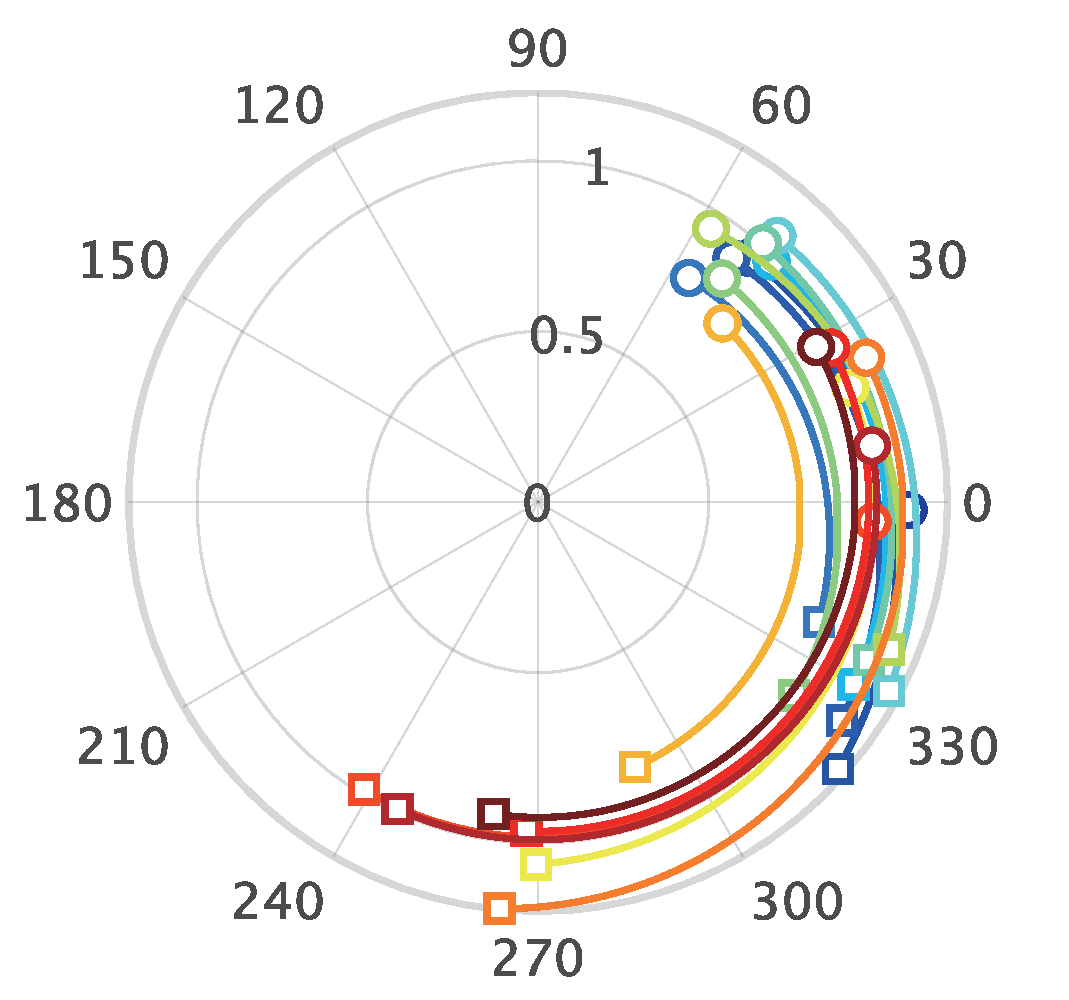
\includegraphics[width = 0.9\linewidth]{figs/Epolar}
    \subcaption{ $E_i e^{\bm{j} \delta_i}$~[pu]}
    \medskip
  \end{minipage}
  \begin{minipage}{0.49\linewidth}
    \centering
    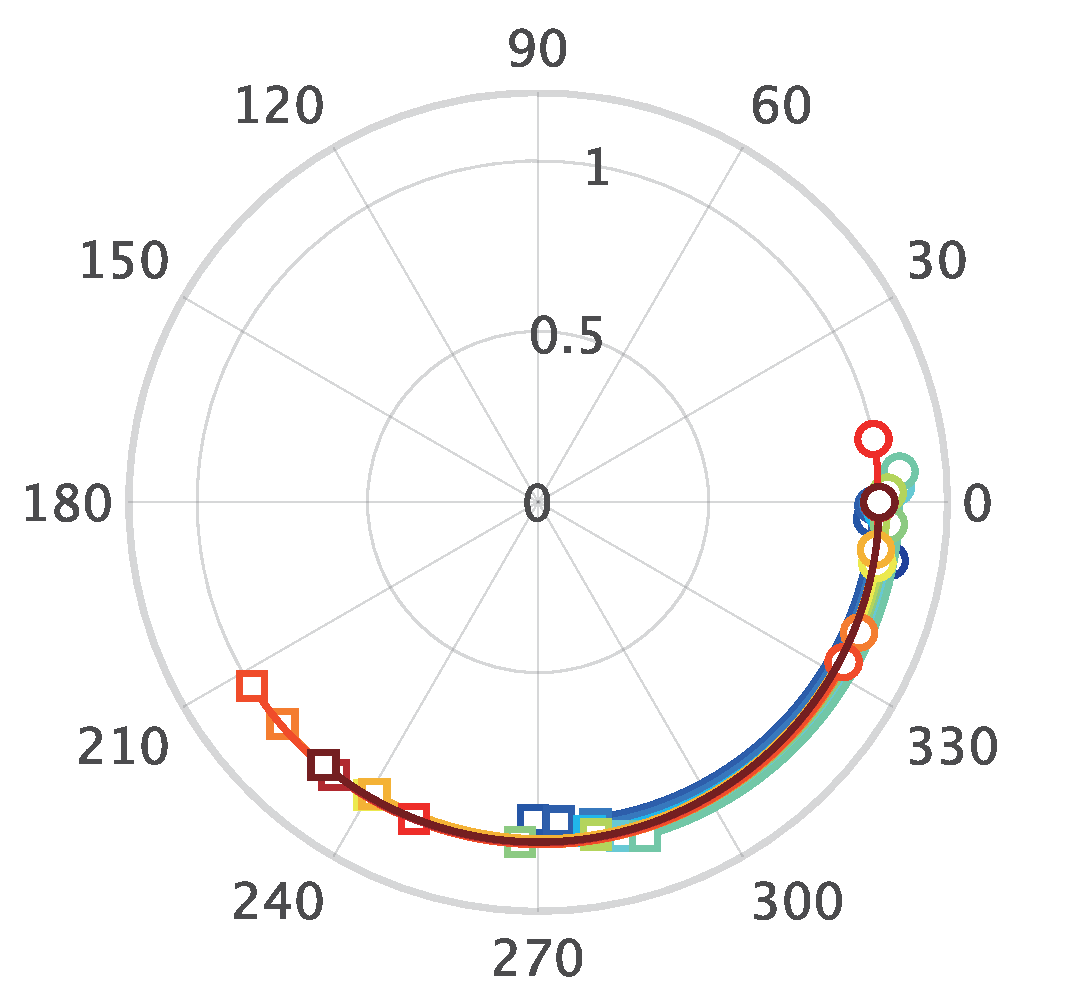
\includegraphics[width = 0.9\linewidth]{figs/Vpolar}
    \subcaption{ $\bm{V}_i$~[pu] }
    \medskip
  \end{minipage}
 \begin{minipage}{0.49\linewidth}
    \centering
    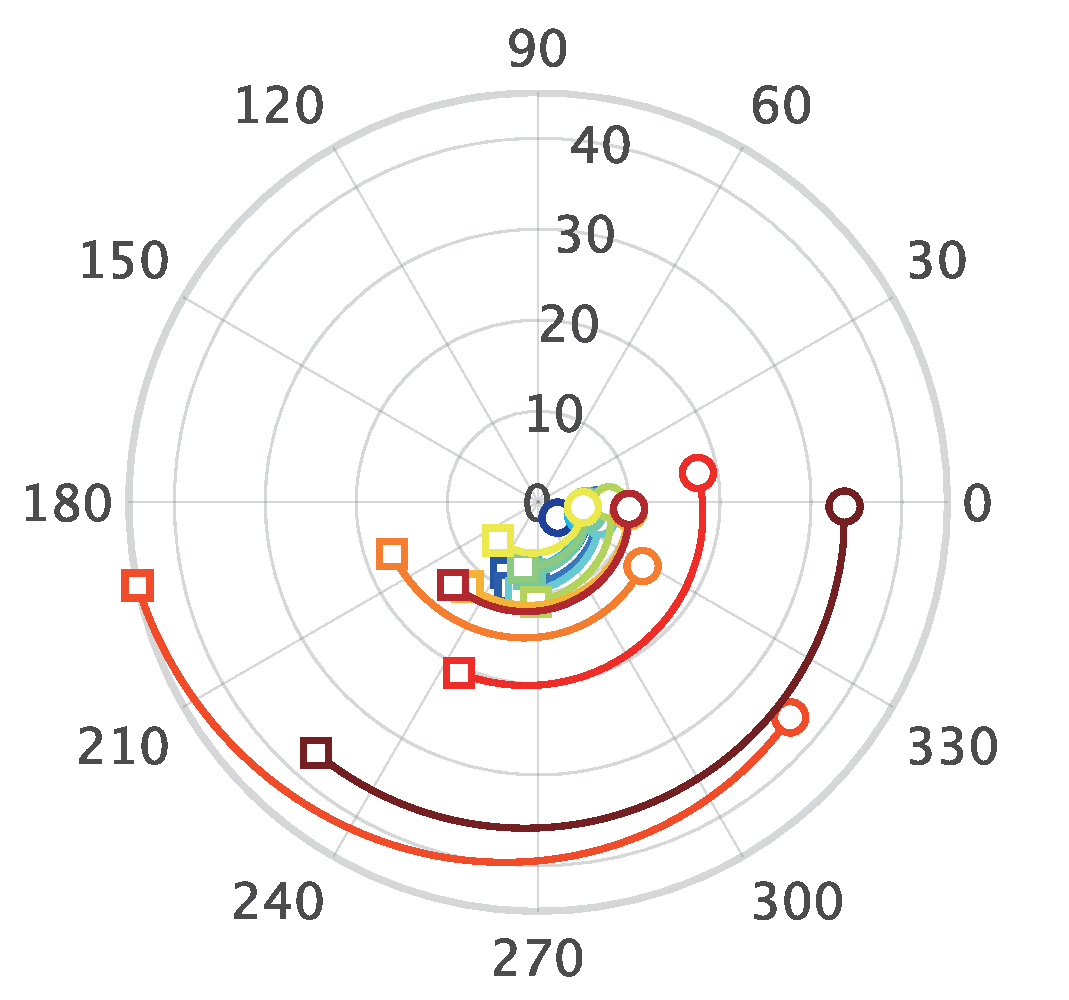
\includegraphics[width = 0.9\linewidth]{figs/Ipolar}
    \subcaption{ $\bm{I}_i$~[pu] }
    \medskip
  \end{minipage}
  \begin{minipage}{0.49\linewidth}
    \centering
    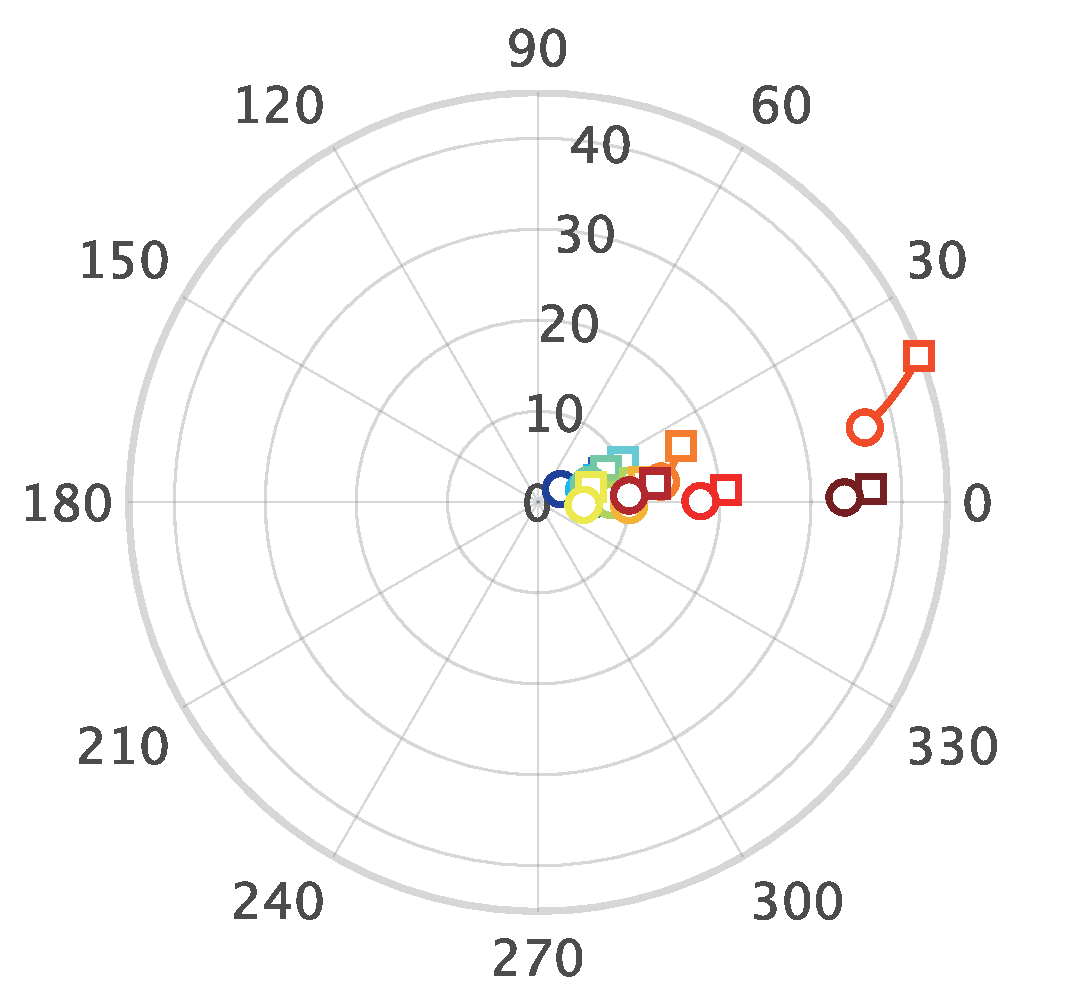
\includegraphics[width = 0.9\linewidth]{figs/PQpolar}
    \subcaption{ $P+\bm{j}Q$~[pu] }
    \medskip
  \end{minipage}
  }
  \medskip
  \caption{\textbf{Changes in generator variables and bus variables with respect to load fluctuations}
  \\  \centering(Circle: initial time, square: end time)}
  \label{fig:polars}
\medskip
\end{figure}


Next, the changes in the generator variable and the bus variable from the initial time to the lapse of 3 hours are shown in \FIGref{fig: polars}.
\FIGref{fig: polars}(a)-(d) are $ E_i e^{\bm{j}\delta_i} $, $ \bm{V}_i $, $ \bm{I}_i $, respectively. , $ P_i + \bm{j} Q_i $ is displayed in polar coordinates on the complex plane.
The value at the initial time $ t = 0 $ is indicated by a circle, and the value at the end time $ t = 10800 $ is indicated by a square.
The following can be read from this figure.

\begin{itemize}
\item \FIGref{fig:polars}(a):The internal voltage of all generators is maintained at a magnitude of 0.7 to 1.5 to [pu], and the rotor declination changes gently clockwise.
\item \FIGref{fig:polars}(b):The absolute value of the bus voltage is maintained in the vicinity of 1 to [pu], and the phase changes slowly clockwise in the same way as the rotor declination.
\item \FIGref{fig:polars}(c):The absolute value of the bus current increases as the power consumption increases with the increase in the impedance value of the load.
\item \FIGref{fig:polars}(d):As the impedance value of the load increases, the active power and reactive power supplied to the bus increase.
\end{itemize}

From the above results, it can be seen that frequency stabilization is properly realized by automatic power generation control.
In addition, it can be seen that the internal state of the generator also changes slowly without vibration in response to gradual load fluctuations, that is, the entire power system is in a quasi-steady state.


\section{Transient stability analysis for generatrix ground faults}\label{sec:IEEE68PSS}

\subsection{Setting of busbar ground fault}

In this section, we analyze the transient stability against bus line ground faults.
The transient stability of the power system is evaluated as follows.
Denote the angular frequency deviation of generator $i$ caused by a ground fault in the busbar $k$ as $\Delta \omega_i^{(k)}$.
The sensitivity of the angular frequency deviation of the entire power system to a ground fault in the busbar $k$ is evaluated by $\|\Delta \omega^{(k)}\|_{\mathcal{L}_2}$.
However, $\Delta \omega^{(k)}$ is a vector of all generator angular frequency deviations $\Delta \omega_1^{(k)},\ldots,\Delta \omega_{16}^{(k)}$.
Also, the set of aligned values of $\|\Delta \omega^{(k)}\|_{\mathcal{L}_2}$ with respect to all generator busbars and load busbars are respectively
\begin{align*}%\label{eq:JGJL}
\mathcal{J}_{\rm G}:=
\left\{
\| \Delta \omega^{(k)} \|_{\mathcal{L}_2}
\right\}_{k\in \{1,\ldots,16\} }
,\qquad
\mathcal{J}_{\rm L}
:=
\left\{
\| \Delta \omega^{(k)} \|_{\mathcal{L}_2}
\right\}_{k\in \{17,\ldots,68\} }
\end{align*}
%\begin{align}\label{eq:JGJL}
%\spliteq{
%\mathcal{J}_{\rm G}
%&:=
%\left\{
%\| \Delta \omega^{(1)} \|_{\mathcal{L}_2}
%,\ldots, 
%\| \Delta \omega^{(16)}\|_{\mathcal{L}_2}
%\right\}
%\\
%\mathcal{J}_{\rm L}
%&:=
%\left\{
%\| \Delta \omega^{(17)} \|_{\mathcal{L}_2}
%,\ldots, 
%\| \Delta \omega^{(68)}\|_{\mathcal{L}_2}
%\right\}
%}
%\end{align}
Considering that ground faults can occur on all bus bars rather than only on a particular bus bar, the high transient stability against bus bar ground faults can be evaluated as the data sets $\mathcal{J}_{\rm G}$ and $\mathcal{J}_{\rm L}$ being small in an appropriate sense.
In this section, $\mathcal{J}_{\rm G}$ and $\mathcal{J}_{\rm L}$ are displayed in a box-and-whisker diagram to visualize the magnitude of the data variability, and their maximum, minimum, and quartiles are used to compare transient stability levels.
Note that the duration of all ground faults should be set to 70~[ms].

\begin{figure}[t!]
  \centering
  {
  \begin{minipage}{0.49\linewidth}
    \centering
    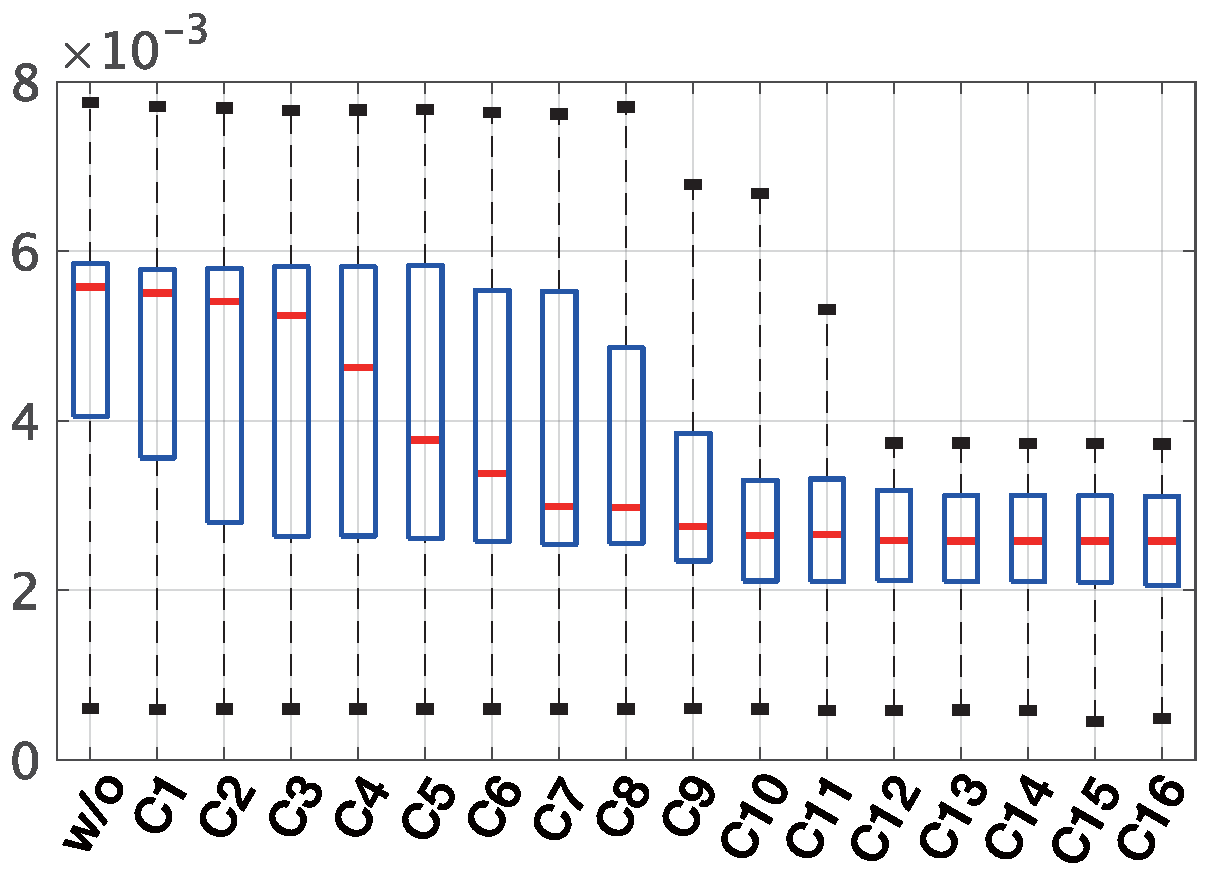
\includegraphics[width = 1.0\linewidth]{figs/boxplotgen}
    \subcaption{ $\mathcal{J}_{\rm G}$: Ground fault in generator bus bar}
  \end{minipage}
  \begin{minipage}{0.49\linewidth}
    \centering
    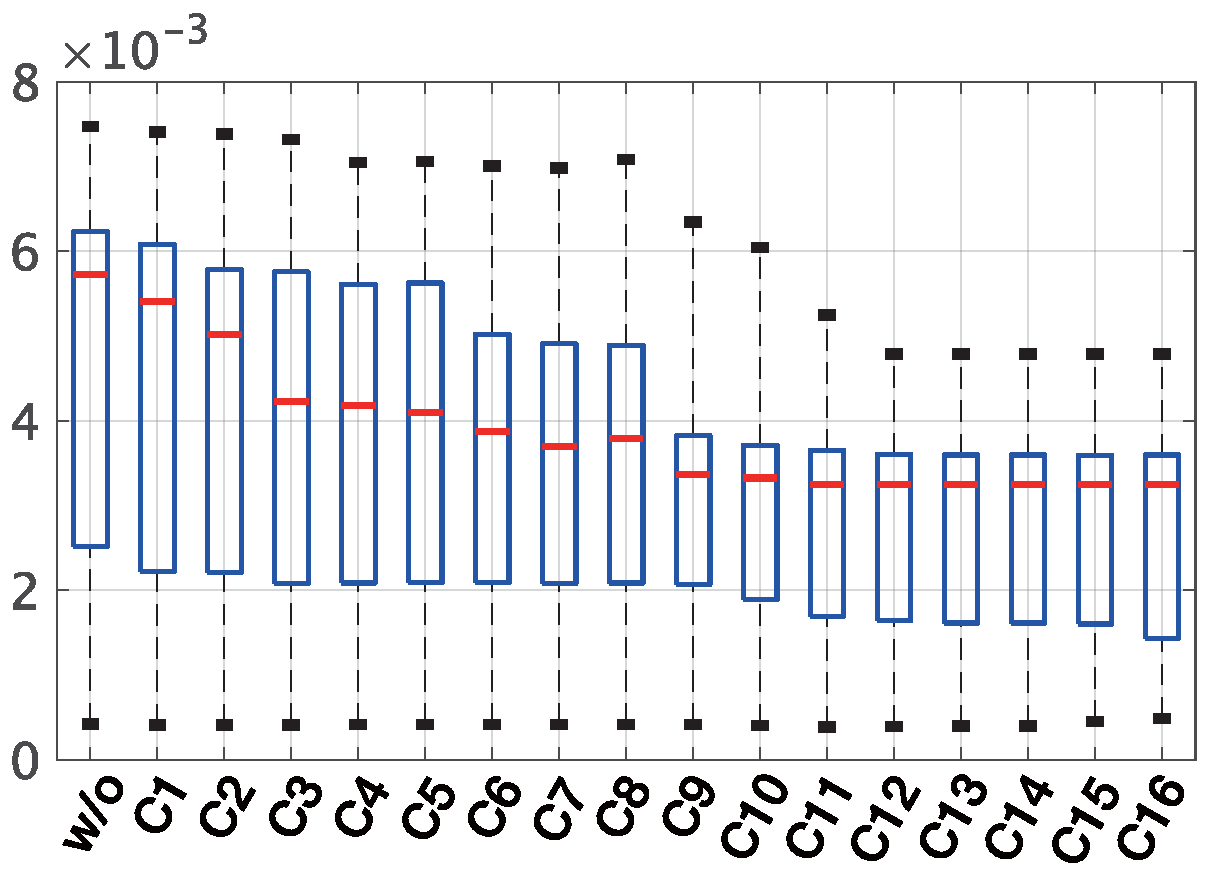
\includegraphics[width = 1.0\linewidth]{figs/boxplotload}
    \subcaption{ $\mathcal{J}_{\rm L}$: load bus bar ground fault}
  \end{minipage}
  \medskip
  \caption{\textbf{Evaluation of system stability against bus-bar ground faults} }
  \label{fig:boxplots}
  }
\medskip
\end{figure}

%\subsection{標準的な自動電圧調整器と系統安定化装置を組み込む場合}

First, we analyze the transient stability when all generators have standard automatic voltage regulators and grid stabilizers built in.
The parameter settings are assumed to be the same as in the \ref{sec:onlyAVR} clause.
The obtained datasets $\mathcal{J}_{\rm G}$ and $\mathcal{J}_{\rm L}$ are displayed as box plots and the results are shown in the first column of the \FIGref{fig:boxplots}.
The \FIGref{fig:boxplots}(a) is the $\mathcal{J}_{\rm G}$ for the earth fault in the generator bus bar and the \FIGref{fig:boxplots}(b) is the $\mathcal{J}_{\rm L}$ for the earth fault in the load bus bar.
In the following, we use these values as a basis to evaluate the improvement in transient stability due to the addition of local controllers.

\subsection{Effectiveness of grid stabilizer based on retrofit control theory}

The transient stability is analyzed when a system stabilizer based on the retrofit control theory described in section \ref{sec:retrofit} is incorporated in each generator.
The retrofit controller incorporated in each generator uses the parameters of the approximate linear environmental model identified from the measurement data by the procedure in the example \ref{ex:modelingV}.
For the local linear subsystem $G_i$, the model of the grid stabilizer is used in addition to the automatic voltage regulator.
The controllers that stabilize the individual design models $G^+_i$ are designed based on the linear quadratic regulator design method described in section \ref{sec:designret}.

The obtained data sets $\mathcal{J}_{\rm G}$ and $\mathcal{J}_{\rm L}$ are displayed as box plots, and the results are shown in columns 2 through 17 of the boxplots of the \FIGref{fig:boxplots}.
The "C$i$" on the horizontal axis represents the case where a retrofit controller is built into each and every generator from generator 1 to generator $i$.
The results show that the degree of grid stability increases step by step with the number of retrofit controllers incorporated.

\begin{table}[h]
\medskip
\caption{\textbf{Physical constants of transmission lines}} \label{table:ieee68lines}
 \centering
  {
  \begin{minipage}{0.49\linewidth}
    \centering
  \begin{tabular}{crrrrcc}
   \hline
$i$--$j$ & $r_{ij}$  &  $x_{ij}$ & $c_{ij}$ \\
   \hline \hline
1--54  & 0 & 0.0181 & 0 \\
2--58  & 0 & 0.0250 & 0 \\
3--62  & 0 & 0.0200 & 0 \\
4--19  & 0.0007 & 0.0142 & 0 \\
5--20  & 0.0009 & 0.0180 & 0 \\
6--22  & 0 & 0.0143 & 0 \\
7--23  & 0.0005 & 0.0272 & 0 \\
8--25  & 0.0006 & 0.0232 & 0 \\
9--29  & 0.0008 & 0.0156 & 0 \\
10--31  & 0 & 0.0260 & 0 \\
11--32  & 0 & 0.0130 & 0 \\
12--36  & 0 & 0.0075 & 0 \\
13--17  & 0 & 0.0033 & 0 \\
14--41  & 0 & 0.0015 & 0 \\
15--42  & 0 & 0.0015 & 0 \\
16--18  & 0 & 0.0030 & 0 \\
17--36  & 0.0005 & 0.0045 & 0.3200 \\
17--43  & 0.0005 & 0.0276 & 0 \\
18--42  & 0.0040 & 0.0600 & 2.2500 \\
18--49  & 0.0076 & 0.1141 & 1.1600 \\
19--20  & 0.0007 & 0.0138 & 0 \\
19--68  & 0.0016 & 0.0195 & 0.3040 \\
21--22  & 0.0008 & 0.0140 & 0.2565 \\
21--68  & 0.0008 & 0.0135 & 0.2548 \\
22--23  & 0.0006 & 0.0096 & 0.1846 \\
23--24  & 0.0022 & 0.0350 & 0.3610 \\
24--68  & 0.0003 & 0.0059 & 0.0680 \\
25--26  & 0.0032 & 0.0323 & 0.5310 \\
25--54  & 0.0070 & 0.0086 & 0.1460 \\
26--27  & 0.0014 & 0.0147 & 0.2396 \\
26--28  & 0.0043 & 0.0474 & 0.7802 \\
26--29  & 0.0057 & 0.0625 & 1.0290 \\
27--37  & 0.0013 & 0.0173 & 0.3216 \\
27--53  & 0.0320 & 0.3200 & 0.4100 \\
28--29  & 0.0014 & 0.0151 & 0.2490 \\
30--31  & 0.0013 & 0.0187 & 0.3330 \\
30--32  & 0.0024 & 0.0288 & 0.4880 \\
30--53  & 0.0008 & 0.0074 & 0.4800 \\
30--61  & 0.0019 & 0.0183 & 0.2900 \\
30--61  & 0.0019 & 0.0183 & 0.2900 \\
31--38  & 0.0011 & 0.0147 & 0.2470 \\
31--53  & 0.0016 & 0.0163 & 0.2500 \\
32--33  & 0.0008 & 0.0099 & 0.1680 \\
\hline
  \end{tabular}
%  \subcaption{データシート}
  \end{minipage}
  \begin{minipage}{0.49\linewidth}
    \centering
  \begin{tabular}{crrrcc}
   \hline
$i$--$j$ & $r_{ij}$  &  $x_{ij}$ & $c_{ij}$ \\
   \hline \hline
33--34  & 0.0011 & 0.0157 & 0.2020 \\
33--38  & 0.0036 & 0.0444 & 0.6930 \\
34--35  & 0.0001 & 0.0074 & 0 \\
34--36  & 0.0033 & 0.0111 & 1.4500 \\
35--45  & 0.0007 & 0.0175 & 1.3900 \\
36--61  & 0.0022 & 0.0196 & 0.3400 \\
36--61  & 0.0022 & 0.0196 & 0.3400 \\
37--52  & 0.0007 & 0.0082 & 0.1319 \\
37--68  & 0.0007 & 0.0089 & 0.1342 \\
38--46  & 0.0022 & 0.0284 & 0.4300 \\
39--44  & 0 & 0.0411 & 0 \\
39--45  & 0 & 0.0839 & 0 \\
40--41  & 0.0060 & 0.0840 & 3.1500 \\
40--48  & 0.0020 & 0.0220 & 1.2800 \\
41--42  & 0.0040 & 0.0600 & 2.2500 \\
43--44  & 0.0001 & 0.0011 & 0 \\
44--45  & 0.0025 & 0.0730 & 0 \\
45--51  & 0.0004 & 0.0105 & 0.7200 \\
46--49  & 0.0018 & 0.0274 & 0.2700 \\
47--48  & 0.0025 & 0.0268 & 0.4000 \\
47--48  & 0.0025 & 0.0268 & 0.4000 \\
47--53  & 0.0013 & 0.0188 & 1.3100 \\
50--51  & 0.0009 & 0.0221 & 1.6200 \\
52--55  & 0.0011 & 0.0133 & 0.2138 \\
53--54  & 0.0035 & 0.0411 & 0.6987 \\
54--55  & 0.0013 & 0.0151 & 0.2572 \\
55--56  & 0.0013 & 0.0213 & 0.2214 \\
56--57  & 0.0008 & 0.0128 & 0.1342 \\
56--66  & 0.0008 & 0.0129 & 0.1382 \\
57--58  & 0.0002 & 0.0026 & 0.0434 \\
58--59  & 0.0006 & 0.0092 & 0.1130 \\
57--60  & 0.0008 & 0.0112 & 0.1476 \\
59--60  & 0.0004 & 0.0046 & 0.0780 \\
60--61  & 0.0023 & 0.0363 & 0.3804 \\
58--63  & 0.0007 & 0.0082 & 0.1389 \\
62--63  & 0.0004 & 0.0043 & 0.0729 \\
62--65  & 0.0004 & 0.0043 & 0.0729 \\
63--64  & 0.0016 & 0.0435 & 0 \\
64--65  & 0.0016 & 0.0435 & 0 \\
65--66  & 0.0009 & 0.0101 & 0.1723 \\
66--67  & 0.0018 & 0.0217 & 0.3660 \\
67--68  & 0.0009 & 0.0094 & 0.1710 \\
\\
   \hline
  \end{tabular}
%   \subcaption{潮流計算結果}
  \end{minipage}
  }
\end{table}


\begin{table}[h]
\medskip
\caption{\textbf{Physical constants of generators}} \label{table:ieee68genpara}
 \centering
 {
\begin{tabular}{crrrrrr}
   \hline
\multicolumn{1}{c}{$i$} & \multicolumn{1}{r}{$M_{i}$} & \multicolumn{1}{r}{$D_{i}$} & \multicolumn{1}{r}{$\tau_{i}$} & \multicolumn{1}{r}{$X_{{\rm d}i}$} & \multicolumn{1}{r}{$X_{{\rm q}i}$} & \multicolumn{1}{r}{$X_{{\rm d}i}'$}  \\
   \hline \hline
1  & \multicolumn{1}{r}{42.0}  & \multicolumn{1}{r}{4.00} & \multicolumn{1}{r}{10.20} & \multicolumn{1}{r}{0.100} & \multicolumn{1}{r}{0.069} & \multicolumn{1}{r}{0.031} \\
2  & \multicolumn{1}{r}{30.2}  & \multicolumn{1}{r}{9.75} & \multicolumn{1}{r}{6.56} & \multicolumn{1}{r}{0.295} & \multicolumn{1}{r}{0.282} & \multicolumn{1}{r}{0.070} \\
3  & \multicolumn{1}{r}{35.8}  & \multicolumn{1}{r}{10.00} & \multicolumn{1}{r}{5.70} & \multicolumn{1}{r}{0.250} & \multicolumn{1}{r}{0.237} & \multicolumn{1}{r}{0.053} \\
4  & \multicolumn{1}{r}{28.6}  & \multicolumn{1}{r}{10.00} & \multicolumn{1}{r}{5.69} & \multicolumn{1}{r}{0.262} & \multicolumn{1}{r}{0.258} & \multicolumn{1}{r}{0.044} \\
5  & \multicolumn{1}{r}{26.0}  & \multicolumn{1}{r}{3.00} & \multicolumn{1}{r}{5.40} & \multicolumn{1}{r}{0.330} & \multicolumn{1}{r}{0.310} & \multicolumn{1}{r}{0.066} \\
6  & \multicolumn{1}{r}{34.8}  & \multicolumn{1}{r}{10.00} & \multicolumn{1}{r}{7.30} & \multicolumn{1}{r}{0.254} & \multicolumn{1}{r}{0.241} & \multicolumn{1}{r}{0.050} \\
7  & \multicolumn{1}{r}{26.4}  & \multicolumn{1}{r}{8.00} & \multicolumn{1}{r}{5.66} & \multicolumn{1}{r}{0.295} & \multicolumn{1}{r}{0.292} & \multicolumn{1}{r}{0.049} \\
8  & \multicolumn{1}{r}{24.3}  & \multicolumn{1}{r}{9.00} & \multicolumn{1}{r}{6.70} & \multicolumn{1}{r}{0.290} & \multicolumn{1}{r}{0.280} & \multicolumn{1}{r}{0.057} \\
9  & \multicolumn{1}{r}{34.5}  & \multicolumn{1}{r}{14.00} & \multicolumn{1}{r}{4.79} & \multicolumn{1}{r}{0.211} & \multicolumn{1}{r}{0.205} & \multicolumn{1}{r}{0.057} \\
10 & \multicolumn{1}{r}{31.0}  & \multicolumn{1}{r}{5.56} & \multicolumn{1}{r}{9.37} & \multicolumn{1}{r}{0.169} & \multicolumn{1}{r}{0.115} & \multicolumn{1}{r}{0.046} \\
11 & \multicolumn{1}{r}{28.2}  & \multicolumn{1}{r}{13.60} & \multicolumn{1}{r}{4.10} & \multicolumn{1}{r}{0.128} & \multicolumn{1}{r}{0.123} & \multicolumn{1}{r}{0.018} \\
12 & \multicolumn{1}{r}{92.3}  & \multicolumn{1}{r}{13.50} & \multicolumn{1}{r}{7.40} & \multicolumn{1}{r}{0.101} & \multicolumn{1}{r}{0.095} & \multicolumn{1}{r}{0.031} \\
13 & \multicolumn{1}{r}{248.0}  & \multicolumn{1}{r}{33.00} & \multicolumn{1}{r}{5.90} & \multicolumn{1}{r}{0.030} & \multicolumn{1}{r}{0.029} & \multicolumn{1}{r}{0.006} \\
14 & \multicolumn{1}{r}{300.0}  & \multicolumn{1}{r}{100.00} & \multicolumn{1}{r}{4.10} & \multicolumn{1}{r}{0.018} & \multicolumn{1}{r}{0.017} & \multicolumn{1}{r}{0.003} \\
15 & \multicolumn{1}{r}{300.0}  & \multicolumn{1}{r}{100.00} & \multicolumn{1}{r}{4.10} & \multicolumn{1}{r}{0.018} & \multicolumn{1}{r}{0.017} & \multicolumn{1}{r}{0.003} \\
16 & \multicolumn{1}{r}{225.0}  & \multicolumn{1}{r}{50.00} & \multicolumn{1}{r}{7.80} & \multicolumn{1}{r}{0.036} & \multicolumn{1}{r}{0.033} & \multicolumn{1}{r}{0.007} \\
\hline
\end{tabular}
}
\end{table}





\begin{table}[h]
\medskip
\caption{\textbf{Datasheet for tidal current calculations (generator bus bar)}} \label{table:ieee68datag}
 \centering
  {
  \begin{minipage}{0.32\linewidth}
    \centering
  \begin{tabular}{crrcc}
   \hline
$i$ & $P_i^{\star}$  &  $|\bm{V}_i^{\star} |$ \\
   \hline \hline
1  & \multicolumn{1}{r}{2.50}   & \multicolumn{1}{r}{1.045} \\
2  & \multicolumn{1}{r}{5.45}   & \multicolumn{1}{r}{0.980} \\
3  & \multicolumn{1}{r}{6.50}   & \multicolumn{1}{r}{0.983} \\
4  & \multicolumn{1}{r}{6.32}   & \multicolumn{1}{r}{0.997} \\
5  & \multicolumn{1}{r}{5.05}   & \multicolumn{1}{r}{1.011} \\
6  & \multicolumn{1}{r}{7.00}   & \multicolumn{1}{r}{1.050} \\
   \hline
  \end{tabular}
%  \subcaption{データシート}
  \end{minipage}
  \begin{minipage}{0.32\linewidth}
    \centering
  \begin{tabular}{ccccc}
   \hline
$i$ & $P_i^{\star}$  &  $|\bm{V}_i^{\star} |$ \\
   \hline \hline
7  & \multicolumn{1}{r}{5.60}   & \multicolumn{1}{r}{1.063} \\
8  & \multicolumn{1}{r}{5.40}   & \multicolumn{1}{r}{1.030} \\
9  & \multicolumn{1}{r}{8.00}   & \multicolumn{1}{r}{1.025} \\
10 & \multicolumn{1}{r}{5.00}   & \multicolumn{1}{r}{1.010} \\
11 & \multicolumn{1}{r}{10.00}   & \multicolumn{1}{r}{1.000} \\
12 & \multicolumn{1}{r}{13.50}   & \multicolumn{1}{r}{1.016} \\
   \hline
  \end{tabular}
%   \subcaption{潮流計算結果}
  \end{minipage}
    \begin{minipage}{0.32\linewidth}
    \centering
  \begin{tabular}{ccccc}
   \hline
$i$ & $P_i^{\star}$  &  $|\bm{V}_i^{\star} |$ \\
   \hline \hline
13  & \multicolumn{1}{r}{35.91}   & \multicolumn{1}{r}{1.011} \\
14  & \multicolumn{1}{r}{17.85}   & \multicolumn{1}{r}{1.000} \\
15  & \multicolumn{1}{r}{10.00}   & \multicolumn{1}{r}{1.000} \\
16  & \multicolumn{1}{r}{40.00}   & \multicolumn{1}{r}{1.000} \\
\\
\\
   \hline
  \end{tabular}
%   \subcaption{潮流計算結果}
  \end{minipage}
  }
\end{table}
 
 
\begin{table}[h]
\medskip
\caption{\textbf{Datasheet used for tidal current calculations (load bus bar)}} \label{table:ieee68datal}
 \centering
  {
  \begin{minipage}{0.32\linewidth}
    \centering
  \begin{tabular}{crrcc}
   \hline
$i$ & $P_i^{\star}$  &  $Q_i^{\star}$ \\
   \hline \hline
\multicolumn{1}{c}{17}  & \multicolumn{1}{r}{$-$60.00} & \multicolumn{1}{r}{$-$3.00} \\
\multicolumn{1}{c}{18}  & \multicolumn{1}{r}{$-$24.70} & \multicolumn{1}{r}{$-$1.23}  \\
\multicolumn{1}{c}{19}  & \multicolumn{1}{r}{0} & \multicolumn{1}{r}{0}  \\
\multicolumn{1}{c}{20}  & \multicolumn{1}{r}{$-$6.80} & \multicolumn{1}{r}{$-$1.03}  \\
\multicolumn{1}{c}{21}  & \multicolumn{1}{r}{$-$2.74} & \multicolumn{1}{r}{$-$1.15}  \\
\multicolumn{1}{c}{22}  & \multicolumn{1}{r}{0} & \multicolumn{1}{r}{0}  \\
\multicolumn{1}{c}{23}  & \multicolumn{1}{r}{$-$2.48} & \multicolumn{1}{r}{$-$0.85} \\
\multicolumn{1}{c}{24}  & \multicolumn{1}{r}{$-$3.09} & \multicolumn{1}{r}{0.92} \\
\multicolumn{1}{c}{25}  & \multicolumn{1}{r}{$-$2.24} & \multicolumn{1}{r}{$-$0.47} \\
\multicolumn{1}{c}{26}  & \multicolumn{1}{r}{$-$1.39} & \multicolumn{1}{r}{$-$0.17}  \\
\multicolumn{1}{c}{27}  & \multicolumn{1}{r}{$-$2.81} & \multicolumn{1}{r}{$-$0.76} \\
\multicolumn{1}{c}{28}  & \multicolumn{1}{r}{$-$2.06} & \multicolumn{1}{r}{$-$0.28}  \\
\multicolumn{1}{c}{29}  & \multicolumn{1}{r}{$-$2.84} & \multicolumn{1}{r}{$-$0.27}  \\
\multicolumn{1}{c}{30}  & \multicolumn{1}{r}{0} & \multicolumn{1}{r}{0} \\
\multicolumn{1}{c}{31}  & \multicolumn{1}{r}{0} & \multicolumn{1}{r}{0} \\
\multicolumn{1}{c}{32}  & \multicolumn{1}{r}{0} & \multicolumn{1}{r}{0} \\
\multicolumn{1}{c}{33}  & \multicolumn{1}{r}{$-$1.12} & \multicolumn{1}{r}{0} \\
\multicolumn{1}{c}{34}  & \multicolumn{1}{r}{0} & \multicolumn{1}{r}{0} \\
   \hline
  \end{tabular}
%  \subcaption{データシート}
  \end{minipage}
  \begin{minipage}{0.32\linewidth}
    \centering
  \begin{tabular}{crrcc}
   \hline
$i$ & $P_i^{\star}$  &  $Q_i^{\star}$ \\
   \hline \hline
\multicolumn{1}{c}{35}  & \multicolumn{1}{r}{0} & \multicolumn{1}{r}{0} \\
\multicolumn{1}{c}{36}  & \multicolumn{1}{r}{$-$1.02} & \multicolumn{1}{r}{0.19} \\
\multicolumn{1}{c}{37}  & \multicolumn{1}{r}{0} & \multicolumn{1}{r}{0} \\
\multicolumn{1}{c}{38}  & \multicolumn{1}{r}{0} & \multicolumn{1}{r}{0} \\
\multicolumn{1}{c}{39}  & \multicolumn{1}{r}{$-$2.67} & \multicolumn{1}{r}{$-$0.13} \\
\multicolumn{1}{c}{40}  & \multicolumn{1}{r}{$-$0.65} & \multicolumn{1}{r}{$-$0.24} \\
\multicolumn{1}{c}{41}  & \multicolumn{1}{r}{$-$10.00} & \multicolumn{1}{r}{$-$2.50} \\
\multicolumn{1}{c}{42}  & \multicolumn{1}{r}{$-$11.50} & \multicolumn{1}{r}{$-$2.50} \\
\multicolumn{1}{c}{43}  & \multicolumn{1}{r}{0} & \multicolumn{1}{r}{0} \\
\multicolumn{1}{c}{44}  & \multicolumn{1}{r}{$-$2.68} & \multicolumn{1}{r}{$-$0.05} \\
\multicolumn{1}{c}{45}  & \multicolumn{1}{r}{$-$2.08} & \multicolumn{1}{r}{$-$0.21} \\
\multicolumn{1}{c}{46}  & \multicolumn{1}{r}{$-$1.51} & \multicolumn{1}{r}{$-$0.29} \\
\multicolumn{1}{c}{47}  & \multicolumn{1}{r}{$-$2.03} & \multicolumn{1}{r}{$-$0.33} \\
\multicolumn{1}{c}{48}  & \multicolumn{1}{r}{$-$2.41} & \multicolumn{1}{r}{$-$0.02} \\
\multicolumn{1}{c}{49}  & \multicolumn{1}{r}{$-$1.64} & \multicolumn{1}{r}{$-$0.29} \\
\multicolumn{1}{c}{50}  & \multicolumn{1}{r}{$-$1.00} & \multicolumn{1}{r}{1.47} \\
\multicolumn{1}{c}{51}  & \multicolumn{1}{r}{$-$3.37} & \multicolumn{1}{r}{1.22} \\
\multicolumn{1}{c}{52}  & \multicolumn{1}{r}{$-$1.58} & \multicolumn{1}{r}{$-$0.30} \\
   \hline
  \end{tabular}
%   \subcaption{潮流計算結果}
  \end{minipage}
    \begin{minipage}{0.32\linewidth}
    \centering
  \begin{tabular}{crrcc}
   \hline
$i$ & $P_i^{\star}$  &  $Q_i^{\star}$ \\
   \hline \hline
\multicolumn{1}{c}{53}  & \multicolumn{1}{r}{$-$2.52} & \multicolumn{1}{r}{$-$1.19} \\
\multicolumn{1}{c}{54}  & \multicolumn{1}{r}{0} & \multicolumn{1}{r}{0} \\
\multicolumn{1}{c}{55}  & \multicolumn{1}{r}{$-$3.22} & \multicolumn{1}{r}{$-$0.02} \\
\multicolumn{1}{c}{56}  & \multicolumn{1}{r}{$-$2.00} & \multicolumn{1}{r}{$-$0.74} \\
\multicolumn{1}{c}{57}  & \multicolumn{1}{r}{0} & \multicolumn{1}{r}{0} \\
\multicolumn{1}{c}{58}  & \multicolumn{1}{r}{0} & \multicolumn{1}{r}{0} \\
\multicolumn{1}{c}{59}  & \multicolumn{1}{r}{$-$2.34} & \multicolumn{1}{r}{$-$0.84} \\
\multicolumn{1}{c}{60}  & \multicolumn{1}{r}{$-$2.09} & \multicolumn{1}{r}{$-$0.71} \\
\multicolumn{1}{c}{61}  & \multicolumn{1}{r}{$-$1.04} & \multicolumn{1}{r}{$-$1.25} \\
\multicolumn{1}{c}{62}  & \multicolumn{1}{r}{0} & \multicolumn{1}{r}{0} \\
\multicolumn{1}{c}{63}  & \multicolumn{1}{r}{0} & \multicolumn{1}{r}{0} \\
\multicolumn{1}{c}{64}  & \multicolumn{1}{r}{$-$0.09} & \multicolumn{1}{r}{$-$0.88} \\
\multicolumn{1}{c}{65}  & \multicolumn{1}{r}{0} & \multicolumn{1}{r}{0} \\
\multicolumn{1}{c}{66}  & \multicolumn{1}{r}{0} & \multicolumn{1}{r}{0} \\
\multicolumn{1}{c}{67}  & \multicolumn{1}{r}{$-$3.20} & \multicolumn{1}{r}{$-$1.53} \\
\multicolumn{1}{c}{68}  & \multicolumn{1}{r}{$-$3.29} & \multicolumn{1}{r}{$-$0.32} \\
\\
\\
   \hline
  \end{tabular}
%   \subcaption{潮流計算結果}
  \end{minipage}
  }
\end{table}







\begin{table}[h]
\medskip
\caption{\textbf{Load impedance}} \label{table:ieee68loads}
 \centering
  {
  \begin{minipage}{0.32\linewidth}
    \centering
  \begin{tabular}{crrcc}
   \hline
$i$ & $r_{{\rm load}i}$  &  $x_{{\rm load}i}$ \\
   \hline \hline
\multicolumn{1}{c}{17}  & \multicolumn{1}{r}{$-$60.00} & \multicolumn{1}{r}{$-$3.00} \\
\multicolumn{1}{c}{18}  & \multicolumn{1}{r}{$-$24.70} & \multicolumn{1}{r}{$-$1.23}  \\
\multicolumn{1}{c}{19}  & \multicolumn{1}{r}{0} & \multicolumn{1}{r}{0}  \\
\multicolumn{1}{c}{20}  & \multicolumn{1}{r}{$-$6.80} & \multicolumn{1}{r}{$-$1.03}  \\
\multicolumn{1}{c}{21}  & \multicolumn{1}{r}{$-$2.74} & \multicolumn{1}{r}{$-$1.15}  \\
\multicolumn{1}{c}{22}  & \multicolumn{1}{r}{0} & \multicolumn{1}{r}{0}  \\
\multicolumn{1}{c}{23}  & \multicolumn{1}{r}{$-$2.48} & \multicolumn{1}{r}{$-$0.85} \\
\multicolumn{1}{c}{24}  & \multicolumn{1}{r}{$-$3.09} & \multicolumn{1}{r}{0.92} \\
\multicolumn{1}{c}{25}  & \multicolumn{1}{r}{$-$2.24} & \multicolumn{1}{r}{$-$0.47} \\
\multicolumn{1}{c}{26}  & \multicolumn{1}{r}{$-$1.39} & \multicolumn{1}{r}{$-$0.17}  \\
\multicolumn{1}{c}{27}  & \multicolumn{1}{r}{$-$2.81} & \multicolumn{1}{r}{$-$0.76} \\
\multicolumn{1}{c}{28}  & \multicolumn{1}{r}{$-$2.06} & \multicolumn{1}{r}{$-$0.28}  \\
\multicolumn{1}{c}{29}  & \multicolumn{1}{r}{$-$2.84} & \multicolumn{1}{r}{$-$0.27}  \\
\multicolumn{1}{c}{30}  & \multicolumn{1}{r}{0} & \multicolumn{1}{r}{0} \\
\multicolumn{1}{c}{31}  & \multicolumn{1}{r}{0} & \multicolumn{1}{r}{0} \\
\multicolumn{1}{c}{32}  & \multicolumn{1}{r}{0} & \multicolumn{1}{r}{0} \\
\multicolumn{1}{c}{33}  & \multicolumn{1}{r}{$-$1.12} & \multicolumn{1}{r}{0} \\
\multicolumn{1}{c}{34}  & \multicolumn{1}{r}{0} & \multicolumn{1}{r}{0} \\
   \hline
  \end{tabular}
%  \subcaption{データシート}
  \end{minipage}
  \begin{minipage}{0.32\linewidth}
    \centering
  \begin{tabular}{crrcc}
   \hline
$i$ & $r_{{\rm load}i}$  &  $x_{{\rm load}i}$ \\
   \hline \hline
\multicolumn{1}{c}{35}  & \multicolumn{1}{r}{0} & \multicolumn{1}{r}{0} \\
\multicolumn{1}{c}{36}  & \multicolumn{1}{r}{$-$1.02} & \multicolumn{1}{r}{0.19} \\
\multicolumn{1}{c}{37}  & \multicolumn{1}{r}{0} & \multicolumn{1}{r}{0} \\
\multicolumn{1}{c}{38}  & \multicolumn{1}{r}{0} & \multicolumn{1}{r}{0} \\
\multicolumn{1}{c}{39}  & \multicolumn{1}{r}{$-$2.67} & \multicolumn{1}{r}{$-$0.13} \\
\multicolumn{1}{c}{40}  & \multicolumn{1}{r}{$-$0.65} & \multicolumn{1}{r}{$-$0.24} \\
\multicolumn{1}{c}{41}  & \multicolumn{1}{r}{$-$10.00} & \multicolumn{1}{r}{$-$2.50} \\
\multicolumn{1}{c}{42}  & \multicolumn{1}{r}{$-$11.50} & \multicolumn{1}{r}{$-$2.50} \\
\multicolumn{1}{c}{43}  & \multicolumn{1}{r}{0} & \multicolumn{1}{r}{0} \\
\multicolumn{1}{c}{44}  & \multicolumn{1}{r}{$-$2.68} & \multicolumn{1}{r}{$-$0.05} \\
\multicolumn{1}{c}{45}  & \multicolumn{1}{r}{$-$2.08} & \multicolumn{1}{r}{$-$0.21} \\
\multicolumn{1}{c}{46}  & \multicolumn{1}{r}{$-$1.51} & \multicolumn{1}{r}{$-$0.29} \\
\multicolumn{1}{c}{47}  & \multicolumn{1}{r}{$-$2.03} & \multicolumn{1}{r}{$-$0.33} \\
\multicolumn{1}{c}{48}  & \multicolumn{1}{r}{$-$2.41} & \multicolumn{1}{r}{$-$0.02} \\
\multicolumn{1}{c}{49}  & \multicolumn{1}{r}{$-$1.64} & \multicolumn{1}{r}{$-$0.29} \\
\multicolumn{1}{c}{50}  & \multicolumn{1}{r}{$-$1.00} & \multicolumn{1}{r}{1.47} \\
\multicolumn{1}{c}{51}  & \multicolumn{1}{r}{$-$3.37} & \multicolumn{1}{r}{1.22} \\
\multicolumn{1}{c}{52}  & \multicolumn{1}{r}{$-$1.58} & \multicolumn{1}{r}{$-$0.30} \\
   \hline
  \end{tabular}
%   \subcaption{潮流計算結果}
  \end{minipage}
    \begin{minipage}{0.32\linewidth}
    \centering
  \begin{tabular}{crrcc}
   \hline
$i$ & $r_{{\rm load}i}$  &  $x_{{\rm load}i}$ \\
   \hline \hline
\multicolumn{1}{c}{53}  & \multicolumn{1}{r}{$-$2.52} & \multicolumn{1}{r}{$-$1.19} \\
\multicolumn{1}{c}{54}  & \multicolumn{1}{r}{0} & \multicolumn{1}{r}{0} \\
\multicolumn{1}{c}{55}  & \multicolumn{1}{r}{$-$3.22} & \multicolumn{1}{r}{$-$0.02} \\
\multicolumn{1}{c}{56}  & \multicolumn{1}{r}{$-$2.00} & \multicolumn{1}{r}{$-$0.74} \\
\multicolumn{1}{c}{57}  & \multicolumn{1}{r}{0} & \multicolumn{1}{r}{0} \\
\multicolumn{1}{c}{58}  & \multicolumn{1}{r}{0} & \multicolumn{1}{r}{0} \\
\multicolumn{1}{c}{59}  & \multicolumn{1}{r}{$-$2.34} & \multicolumn{1}{r}{$-$0.84} \\
\multicolumn{1}{c}{60}  & \multicolumn{1}{r}{$-$2.09} & \multicolumn{1}{r}{$-$0.71} \\
\multicolumn{1}{c}{61}  & \multicolumn{1}{r}{$-$1.04} & \multicolumn{1}{r}{$-$1.25} \\
\multicolumn{1}{c}{62}  & \multicolumn{1}{r}{0} & \multicolumn{1}{r}{0} \\
\multicolumn{1}{c}{63}  & \multicolumn{1}{r}{0} & \multicolumn{1}{r}{0} \\
\multicolumn{1}{c}{64}  & \multicolumn{1}{r}{$-$0.09} & \multicolumn{1}{r}{$-$0.88} \\
\multicolumn{1}{c}{65}  & \multicolumn{1}{r}{0} & \multicolumn{1}{r}{0} \\
\multicolumn{1}{c}{66}  & \multicolumn{1}{r}{0} & \multicolumn{1}{r}{0} \\
\multicolumn{1}{c}{67}  & \multicolumn{1}{r}{$-$3.20} & \multicolumn{1}{r}{$-$1.53} \\
\multicolumn{1}{c}{68}  & \multicolumn{1}{r}{$-$3.29} & \multicolumn{1}{r}{$-$0.32} \\
\\
\\
   \hline
  \end{tabular}
%   \subcaption{潮流計算結果}
  \end{minipage}
  }
\end{table}

\newpage
%\printindex
%
%
\end{document}